\documentclass[14pt, a4paper]{article}
\usepackage{minitoc}
\usepackage[left=3.00cm, right=2.5cm, top=2.00cm, bottom=2.00cm]{geometry}
\usepackage{amsmath}
\usepackage{amssymb}
\usepackage{amsthm}
\usepackage{mathtools}
\usepackage{graphicx}
%\usepackage{algpseudocode}
%\usepackage{algorithm}
\usepackage[ruled,vlined,linesnumbered]{algorithm2e}
\usepackage{blindtext}
\usepackage{setspace}
\usepackage[utf8]{inputenc}
\usepackage[utf8]{vietnam}
\usepackage[center]{caption}
\usepackage[shortlabels]{enumitem}
\usepackage{fancyhdr} % header, footer
\usepackage{hyperref} % loại bỏ border với mục lục và công thức
\usepackage[nonumberlist, nopostdot, nogroupskip]{glossaries}
\usepackage{glossary-superragged}
\usepackage{tikz,tkz-tab}
\usepackage{pythonhighlight}
\setglossarystyle{superraggedheaderborder}
\pagestyle{fancy}
%\usepackage[style=numeric,sortcites]{biblatex}
%\addbibresource{ref.bib}
%\usepackage[numbers]{natbib}
\usepackage{indentfirst}
\usepackage[natbib,backend=biber,style=ieee, sorting=ynt]{biblatex}
\bibliography{ref.bib}

\graphicspath{{./figures/}}

\fancyhf{}
%\rhead{\textbf{Môn học: Các phương pháp thống kê hiện đại trong nghiên cứu Xã hội học}}
\lhead{\textbf{GVHD: TS. Trịnh Quốc Anh}}
\rfoot{\thepage}
\lfoot{\textbf{Học viên thực hiện: Nguyễn Chí Thanh - 21007925}}
\renewcommand{\headrulewidth}{0.4pt}
\renewcommand{\footrulewidth}{0.4pt}
%
%\numberwithin{equation}{section}
%\numberwithin{algorithm}{section}
%\numberwithin{figure}{section}
%
%\setlength{\parindent}{0.5cm}
%
%\setcounter{secnumdepth}{3} % Cho phép subsubsection trong report
%\setcounter{tocdepth}{3} % Chèn subsubsection vào bảng mục lục

%\newtheorem{dl}{Định lý}
%\newtheorem{md}{Mệnh đề}
%\newtheorem{bd}{Bổ đề}
%\newtheorem{dn}{Định nghĩa}
%\newtheorem{hq}{Hệ quả}

%\newtheorem{baitap}{Bài tập}
%\newtheorem*{loigiai}{Lời giải}

%\numberwithin{dl}{section}
%\numberwithin{md}{section}
%\numberwithin{bd}{section}
%\numberwithin{dn}{section}
%\numberwithin{hq}{section}

\setlength{\parindent}{0cm}

\newtheorem{dl}{Định lý}
\newtheoremstyle{sltheorem}
{}                % Space above
{}                % Space below
{\normalfont}        % Theorem body font % (default is "\upshape")
{}                % Indent amount
{\bfseries}       % Theorem head font % (default is \mdseries)
{.}               % Punctuation after theorem head % default: no punctuation
{ }               % Space after theorem head
{}                % Theorem head spec
\theoremstyle{sltheorem}
\newtheorem{baitap}{Bài tập}
\newtheoremstyle{soltheorem}
{}                % Space above
{}                % Space below
{\normalfont}        % Theorem body font % (default is "\upshape")
{}                % Indent amount
{\bfseries}       % Theorem head font % (default is \mdseries)
{.}               % Punctuation after theorem head % default: no punctuation
{\newline}               % Space after theorem head
{}                % Theorem head spec
\theoremstyle{soltheorem}
\newtheorem*{loigiai}{Lời giải}

\onehalfspacing


\begin{document}
\begin{titlepage}

    \newcommand{\HRule}{\rule{\linewidth}{0.5mm}} % Defines a new command for the horizontal lines, change thickness here

    \center % Center everything on the page

    %----------------------------------------------------------------------------------------
    %	HEADING SECTIONS
    %----------------------------------------------------------------------------------------
    \textsc{\LARGE Đại học Quốc Gia Hà Nội}\\[0.5cm]
    \textsc{\LARGE Trường đại học Khoa học tự nhiên}\\[0.5cm] % Name of your university/college
    \textsc{\LARGE Khoa Toán - Cơ - Tin học}\\[0.5cm]

    
\includegraphics[scale=0.2]{HUS-logo.jpg}\\[0.5cm]

    \textsc{\Large Chuyên ngành: Khoa học dữ liệu}\\[0.5cm] % Major heading such as course name


    %----------------------------------------------------------------------------------------
    %	TITLE SECTION
    %----------------------------------------------------------------------------------------

    \HRule \\[0.4cm]
    { \huge \bfseries Bài tập môn học}\\[0.4cm] % Title of your document
    \HRule \\[1.5cm]

    \textsc{\Large Môn học: Các phương pháp thống kê hiện đại \\ trong nghiên cứu Xã hội học}\\[1cm] % Minor heading such as course title


    \textsc{\Large Bài tập 1}\\[1cm]


    %----------------------------------------------------------------------------------------
    %	AUTHOR SECTION
    %----------------------------------------------------------------------------------------
    \begin{minipage}{0.4\textwidth}
        \begin{flushleft} \large
        \emph{Giảng viên hướng dẫn:} \\
        TS. Trịnh Quốc Anh % Supervisor's Name
        \end{flushleft}
    \end{minipage}\\[0.5cm]

    \begin{minipage}{0.4\textwidth}
    \begin{flushleft} \large
    \emph{Học viên thực hiện:}\\
    Nguyễn Chí Thanh \\
    MSHV: 21007925 \\ % Your name
    Lớp: Khoa học dữ liệu - K4
    \end{flushleft}
    \end{minipage}


    % If you don't want a supervisor, uncomment the two lines below and remove the section above
    %\Large \emph{Author:}\\
    %John \textsc{Smith}\\[3cm] % Your name

    %----------------------------------------------------------------------------------------
    %	DATE SECTION
    %----------------------------------------------------------------------------------------

    % I don't want day because it is English
    % {\large \today}\\[2cm] % Date, change the \today to a set date if you want to be precise

    %----------------------------------------------------------------------------------------
    %	LOGO SECTION
    %----------------------------------------------------------------------------------------

    %\includegraphics{logo/rsz_3logo-khtn.png}\\[1cm] % Include a department/university logo - this will require the graphicx package

    %----------------------------------------------------------------------------------------

    \vfill % Fill the rest of the page with whitespace

\end{titlepage}

\nocite{*}

\newpage


\begin{baitap}
    Trả lời các câu hỏi 1 - 12, của quyển sách \cite{nolan2001stat}, trang 21 - 23
\end{baitap}

\begin{loigiai}
    Trả lời các câu hỏi 1 - 12, của quyển sách \cite{nolan2001stat}, trang 21 - 23
    \begin{enumerate}[wide, labelwidth=!, labelindent=0pt,label=\textbf{\arabic*}.]
        \item Sử dụng bảng \ref{tb:1.3} để ước lượng các phân vị phần tư của phân phối của số điếu thuốc đượt hút một ngày của các bà mẹ hút trong thời gian thai kỳ từ CHDS.

            \begin{table}[h!]
                \begin{center}
                    \begin{tabular}{|c|c|}
                        \hline
                        \textbf{Số điếu thuốc được hút} & \textbf{Tỷ lệ trong số người hút thuốc} \\  
                        \hline
                        0--5 & 16\% \\  
                        5--10 & 25\% \\  
                        10--15 & 14\% \\  
                        15--20 & 4\% \\  
                        20--30 & 32\% \\  
                        30--40 & 5\% \\  
                        40--60 & 4\% \\  
                        \hline
                        Tổng cộng & 100 \% \\
                        \hline
                    \end{tabular}
                \end{center}
                \caption{Bản tần suất của số điếu thuốc được hút trong một ngày của 484 bà mẹ trong tập CHDS có hút thuốc trong thời gian thai kỳ,
                tỷ lệ phần trăm được làm tròn đến số nguyên gần nhất}
                \label{tb:1.3}
            \end{table}
        
        Ta có:
        \begin{equation*}
            \begin{aligned}
                &Q_1 = 5 + \dfrac{10 - 5}{25} \times (25 - 16) = 6.80 \\
                &Q_2 = 10 + \dfrac{15 - 10}{14} \times (50 - 41) = 13.21 \\
                &Q_3 = 20 + \dfrac{30 - 20}{32} \times (75 - 59) = 25
            \end{aligned}
        \end{equation*}

        \item Hợp bốn nhóm cuối trong bảng \ref{tb:1.3} thành một nhóm của phân phối số điếu thuốc đượt hút một ngày của các bà mẹ hút trong thời gian thai kỳ từ CHDS.
        Xây dựng histogram mới từ bảng thu được. Hình dạng thay đổi như nào so với histogram cũ?

        Ta có bảng phân phối mới sau khi hợp bốn nhóm cuối trong bảng \ref{tb:1.3}:

        \begin{table}[h!]
            \begin{center}
                \begin{tabular}{|c|c|}
                    \hline
                    \textbf{Số điếu thuốc được hút} & \textbf{Tỷ lệ trong số người hút thuốc} \\  
                    \hline
                    0--5 & 16\% \\  
                    5--10 & 25\% \\  
                    10--15 & 14\% \\  
                    15--60 & 45\% \\  
                    \hline
                    Tổng cộng & 100 \% \\
                    \hline
                \end{tabular}
            \end{center}
            \caption{Bản tần suất của số điếu thuốc được hút trong một ngày của 484 bà mẹ trong tập CHDS có hút thuốc trong thời gian thai kỳ,
            tỷ lệ phần trăm được làm tròn đến số nguyên gần nhất}
        \end{table}

        Ta sử dụng code để vẽ histogram mới:

        \begin{python}
import numpy as np
import matplotlib.pyplot as plt
            
            
lower = np.array([0, 5, 10, 15])
upper = np.array([5, 10, 15, 60])
            
percent = np.array([16, 25, 14, 45])
            
plt.bar(lower, percent/(upper-lower), width=upper - lower, ec="k", align="edge")
plt.xticks(lower.tolist() + [upper.tolist()[-1]], rotation=45)
plt.xlabel("Number of cigarettes (per day)")
plt.ylabel("Percent per cigarette")
plt.grid()
plt.show()
        \end{python}

        \begin{figure}[h!]
            \centering
            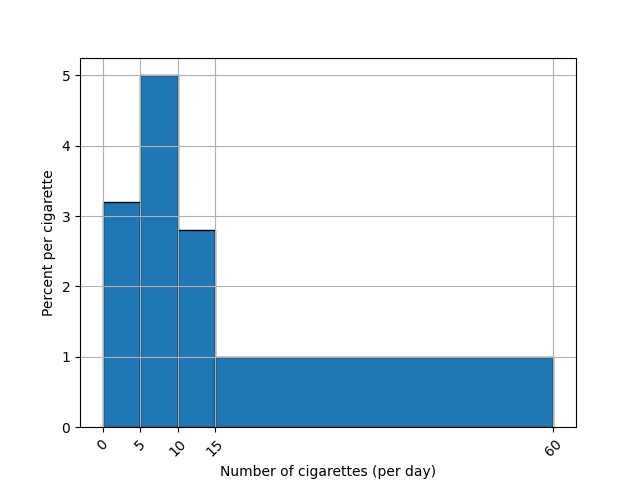
\includegraphics[scale=0.8]{2.png}
            \caption{histogram mới sau khi hợp bốn nhóm cuối bảng \ref{tb:1.3}}
        \end{figure}

        \item Ta xét histogram của tuổi của những người cha trong tập CHDS (hình \ref{fig:1.14}). Cột tương ứng với khoảng tuổi từ 35 đến 40 tuổi bị mất. Tìm chiều cao của cột này.
        \begin{figure}[h!]
            \centering
            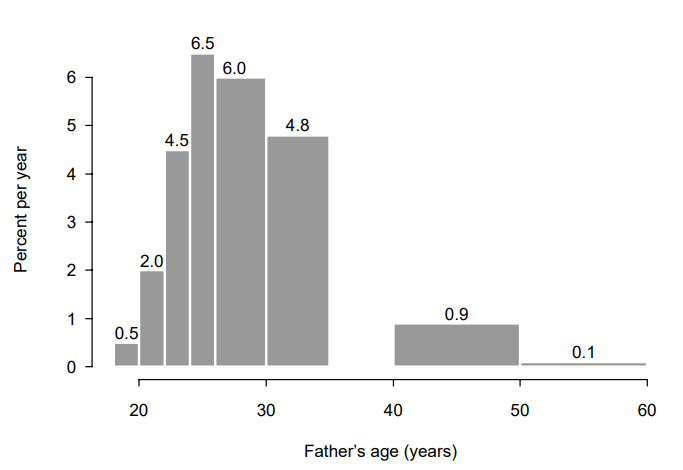
\includegraphics[scale=0.8]{1.14.png}
            \caption{Tuổi của những người cha (năm)}
            \label{fig:1.14}
        \end{figure}

        Ta đặt chiều cao của cột tương ứng với khoảng 35 - 40 tuổi là $x$:

        \begin{equation*}
            \begin{aligned}
                &0.5 \times 20 + 2.0 \times 2 + 4.5 \times 2 + 6.5 \times 2 + 6.0 \times 4 + 4.8 \times 5 + x \times 5 + 0.9 \times 10 + 0.1\times 10 = 100 \\
                &\Rightarrow x = \dfrac{100 - (0.5 \times 20 + 2.0 \times 2 + 4.5 \times 2 + 6.5 \times 2 + 6.0 \times 4 + 4.8 \times 5 + 0.9 \times 10 + 0.1\times 10)}{5} = \dfrac{100-94}{5}=1.2 \%
            \end{aligned}
        \end{equation*}

        Vậy chiều cao của cột tương ứng với khoảng 35 - 40 tuổi là 1.2 \%

        \item Ta xét quantile plot của chiều cao và cân nặng của những người cha trong CHDS (hình \ref{fig:1.15}). Hãy miêu tả hình dạng của các phân phối trên.
        \begin{figure}[h!]
            \centering
            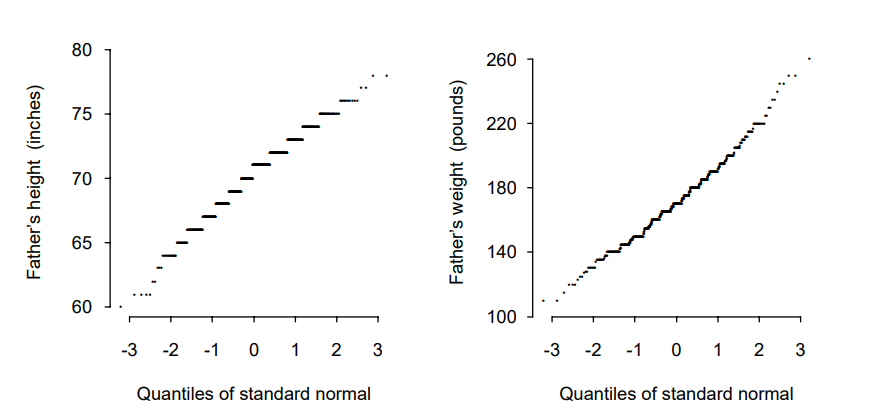
\includegraphics[scale=0.7]{1.15.png}
            \caption{Đồ thị quantile của chiều cao của những người cha (bên trái) và cân nặng (bên phải) trong tập CHDS.}
            \label{fig:1.15}
        \end{figure}

        Đồ thị quantile của chiều cao của những người cha cho thấy chiều cao được đo là một đại lượng rời rạc.
        Ta nhận thấy các điểm gần như nằm trên một đường thẳng cho thấy phân phối chiều cao của những người cha xấp xỉ phân phối chuẩn.
        
        \begin{figure}[h!]
            \centering
            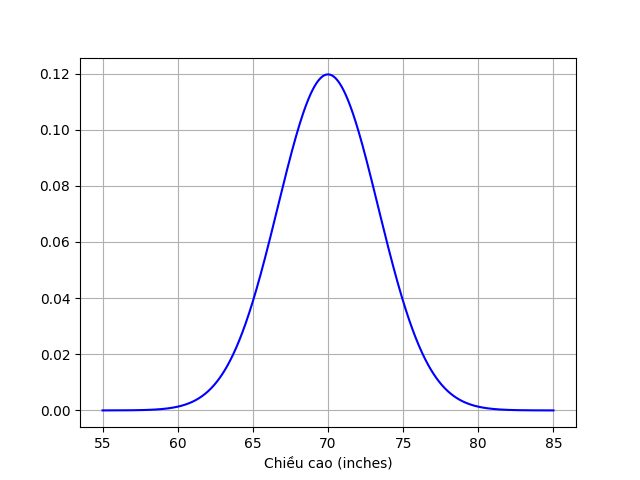
\includegraphics[scale=0.7]{4.1.png}
            \caption{Đồ thị hàm mật độ lý thuyết chiều cao của những người cha}
        \end{figure}

        Đồ thị quantile cân nặng của người cha cho thấy các điểm nằm khá sát trên một đường thẳng nên phân phối có dạng xấp xỉ phân phối chuẩn và phân phối khá đối xứng nhưng có khá ít điểm rơi vào khoảng biên và đa số các điểm tập trung ở khu vực trung nên cho ta thấy phân phối có hai bên đuôi khá nhẹ.
        
        \begin{figure}[h!]
            \centering
            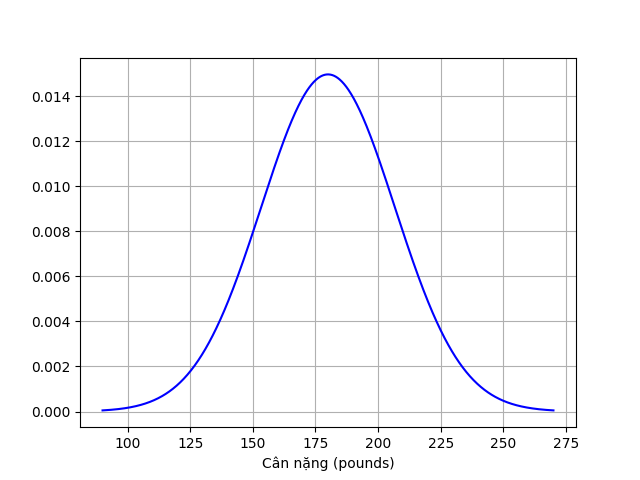
\includegraphics[scale=0.7]{4.2.png}
            \caption{Đồ thị hàm mật độ lý thuyết cân nặng của những người cha}
        \end{figure}

        \item Theo các phân vị 0.05, 0.1, \dots, 0.95 cho thời gian thai kỳ của em bé trong tập CHDS.
        Miêu tả hình dạng của phân phối của thời gian thai kỳ so với phân phối đều.
        252, 262, 267, 270, 272, 274, 276, 277, 278, 280, 281, 283, 284, 286, 288, 290, 292, 296, 302.
        
        Ta sử dụng đoạn code sau để vẽ đồ thị quantile của số liệu trên.

        \begin{python}
import numpy as np 
import pylab 
import scipy.stats as stats
import matplotlib.pyplot as plt
            
measurements = np.array([252, 262, 267, 270, 272, 274, 276, 277, 278, 280, 281, 283, 284, 286, 288, 290, 292, 296, 302])
quantiles = np.arange(1, measurements.shape[0] + 1) / (measurements.shape[0] + 1)
print(quantiles)
#plt.scatter(quantiles, measurements)
#plt.grid()
#plt.show()
stats.probplot(measurements, dist="uniform", plot=pylab)
pylab.title("Quantile plot")
pylab.xlabel("Quantiles of uniform")
pylab.ylabel("Gestational age")
pylab.grid()
pylab.show()
        \end{python}

        \begin{figure}[h!]
            \centering
            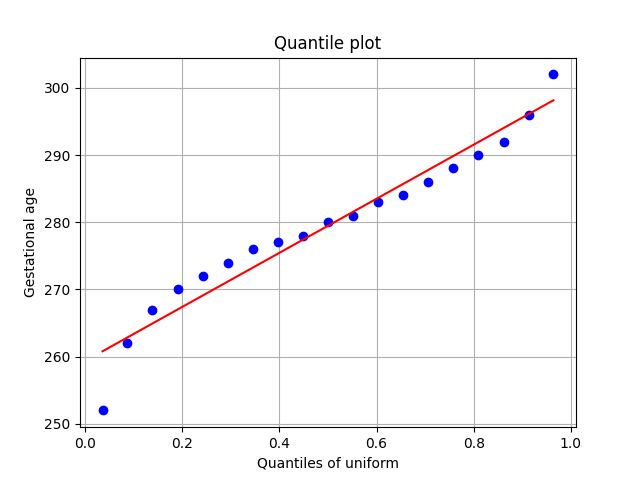
\includegraphics[scale=0.7]{5.png}
            \caption{Đồ thị quantile tương ứng với phân phối dữ liệu thời gian thai kỳ của em bé.}
        \end{figure}
    \end{enumerate}

\end{loigiai}

\newpage
\printbibliography[title={TÀI LIỆU THAM KHẢO}]

\end{document}